\chapter{LAR}
\label{sec:LAR}

LAR is a general representation scheme for geometric and topological
modeling~\cite{Dicarlo:2014:TNL:2543138.2543294}. 
The domain of the scheme is provided by \textit{cellular complexes}
while its codomain is a set of \textit{sparse matrices}.
The main advantages of the scheme are:
\begin{enumerate}
    \item
    \textit{It is extremely effective to easily represent general non-manifold solids.}
    For example, the memory representation of a $d=3$ cellular complex using LAR 
    consists in only two binary sparse matrices for the topology and a bi-dimensional
    array for the geometry.
    \item
    \textit{Computation and analysis of cellular complexes is
    done only through easy linear algebra operations.} 
    The most common operation is the sparse matrix-vector 
    multiplication.
\end{enumerate}

In LAR we talk about cellular complexes which are made of cells, so we
call $d$-cell the $d$-dimensional cell: 0-cells are vertices,
1-cells are edges, 2-cells are faces, and so on.
Throughout this thesis, these names are completely
interchangeable.

An important concept is represented by the \textit{boundary} and 
\textit{coboundary operators}. They express the relation
between the cells of different dimension but of the same cellular complex.
Even these operators are stored in memory as sparse matrices 
and they can be applied using just a matrix multiplication.

The relation $\partial_d = \delta_{d-1}^\top$ (where $\partial_d$ 
is the $d$-boundary and $\delta_{d-1}$ is the $(d-1)$-coboundary)
is particularly handy. So, for example a 2-boundary expresses 
the relation from the edges to the faces of the same complex and
its transpose is the 1-coboundary that maps faces to edges.

An another concept of LAR used a lot in this thesis is the one of
\textit{skeleton}. A $(d-1)$-skeleton is the set of $(d-1)$-cells of
a $d$-complex. For example, a 2-skeleton of a 3-complex is the set
of all the faces of the complex.

\section{LAR fundamentals}
\label{sec:fundamentals}

\paragraph{LAR model}
A LAR model is a pair \emph{geometry, topology}. The \emph{geometry} is specified by the  position vectors of \emph{vertices} in a Euclidean space $\E^d$ of points with $d$ coordinates. The \emph{topology} is specified by one or more bases of singleton $k$-chains (i.e.~$k$-cells) for $0 \leq k\leq d$. The vertex sharing between cells implicitly provide the attachment maps between cells of various dimensions.
Vertex positions are represented, by rows, by a 2-array of d real coordinates.

\paragraph{Chains as arrays}
Chain-based modeling and computing is based on representation of $p$-cell subsets as \emph{chains}, elements of \emph{linear} spaces $C_p$ ($0\leq p\leq d$) generated by the space decomposition induced by a \emph{cellular complex}, also said \emph{CW- complex}.
Chains can be simply represented as arrays of signed integers, one of simplest and more efficient data structure of most languages, particularly when oriented to scientific computing.
Therefore, basic algebraic operations on chains as vectors (sum and product times a scalar) are implemented over arrays.

\paragraph{Characteristic matrices}
The LAR \emph{representation scheme}~\cite{Requicha:1980:RRS:356827.356833}, i.e.~our mapping between mathematical models of solids and their computer representations, uses linear \emph{chain spaces} $C_p$ as models, and sparse \emph{characteristic matrices} $M_p$  of $p$-cells as symbolic representations, where the $p$-cell $\sigma^k\in\Lambda_p$ is represented as the $k$-th binary row of the  sparse characteristic matrix $M_p: C_0\to C_p$.

\paragraph{Boundary and coboundary matrices}

The boundary matrix $[\partial_p]$ is the matrix of the boundary operator $\partial_p: C_p\to C_{p-1}$ ($1\leq p\leq d$) that for each \emph{chain} $c_p\in C_p$ returns the  boundary $(p-1)$-cycle of its $(d-1)$-faces.  A boundary operator is linear: $\partial_p c + d = \partial_p c + \partial_p d$, for each $c,d\in C_p$. A cycle is a chain without boundary. Hence, t\emph{he} boundary of a boundary is the zero map: $partial_{p-1} \circ partial_p = 0$ ($2\leq p\leq d$).

\paragraph{Incidence matrices}
Incidence operators between chain spaces of different dimension are easy to compute by matrix products of characteristic matrices (see Section~\ref{matrices}), possibly transposed.
Since both characteristic and operator matrices are very sparse, their products are computed with  specialized algorithms for very sparse matrices, whose complexity is roughly linear in the size of the output sparse matrix, i.e., in the number of its stored non-zero elements.
Incidence queries and other types of geometric or topological computations are not performed element-wise, that necessarily require iterative or recursive programming patterns, but only require matrix product times whole chains (sets of cells), so adapting naturally to parallel and/or dataflow computational patterns found in HPC and CNN architectures.

\paragraph{Validity test of a representation}
Data validity is easy to test by checking for satisfaction of basic equations $\partial\partial=\emptyset$ of a chain complex.



\section{Historical notes}
\label{sec:history}
LAR has been developed for several years, in a joint collaboration 
between Roma Tre University and the University 
of Wisconsin at Madison \cite{ieee-tase}. The development of a Python 
prototype start in 2012 by A. Paoluzzi but was interrupted 
in December 2016 for various reasons. The development of the current
Julia implementation started few months later (March 2017) with
G. Martella and F. Furiani as main developers. This thesis is
the main core of the Julia implementation.


\section{Literate programming}
This package has been developed using literate programming.
Literate programming is a programming paradigm in which the program
logic is explained in natural language and the code is embedded in macros.
Quoting Donald E. Knuth, the creator of the paradigm: 
\textit{``[Literate programming] allows a person to express programs in a stream of
consciousness order. [...] [Code can] be explored
in a psychologically correct order''} \cite{knuth}. 
With this premise it is easy to understand why literate programming 
is widely used for academic works.
When the goal is to learn and share knowledge, literate programming fits perfectly.


\section{Julia}

Ths implementation has been made in Julia
Julia is a relatively new high-level programming language targeted 
to numerical computing. The project was born back in 2009 and its first
stable version was released in 2012. As stated in the first blog post
on Julia's official website, the language has the goal
to be \textit{``Something that is dirt simple to learn, 
yet keeps the most serious hackers happy''}, with the speed of C, 
the dynamism of Ruby and the distributed power of Hadoop
\cite{julia}.


%%%%%%%%%%%%%%%%%%%%%%%
\chapter{The arrangement algorithm}
\label{ch:arrangement_algorithm}

\begin{figure}[H]
    \centering
    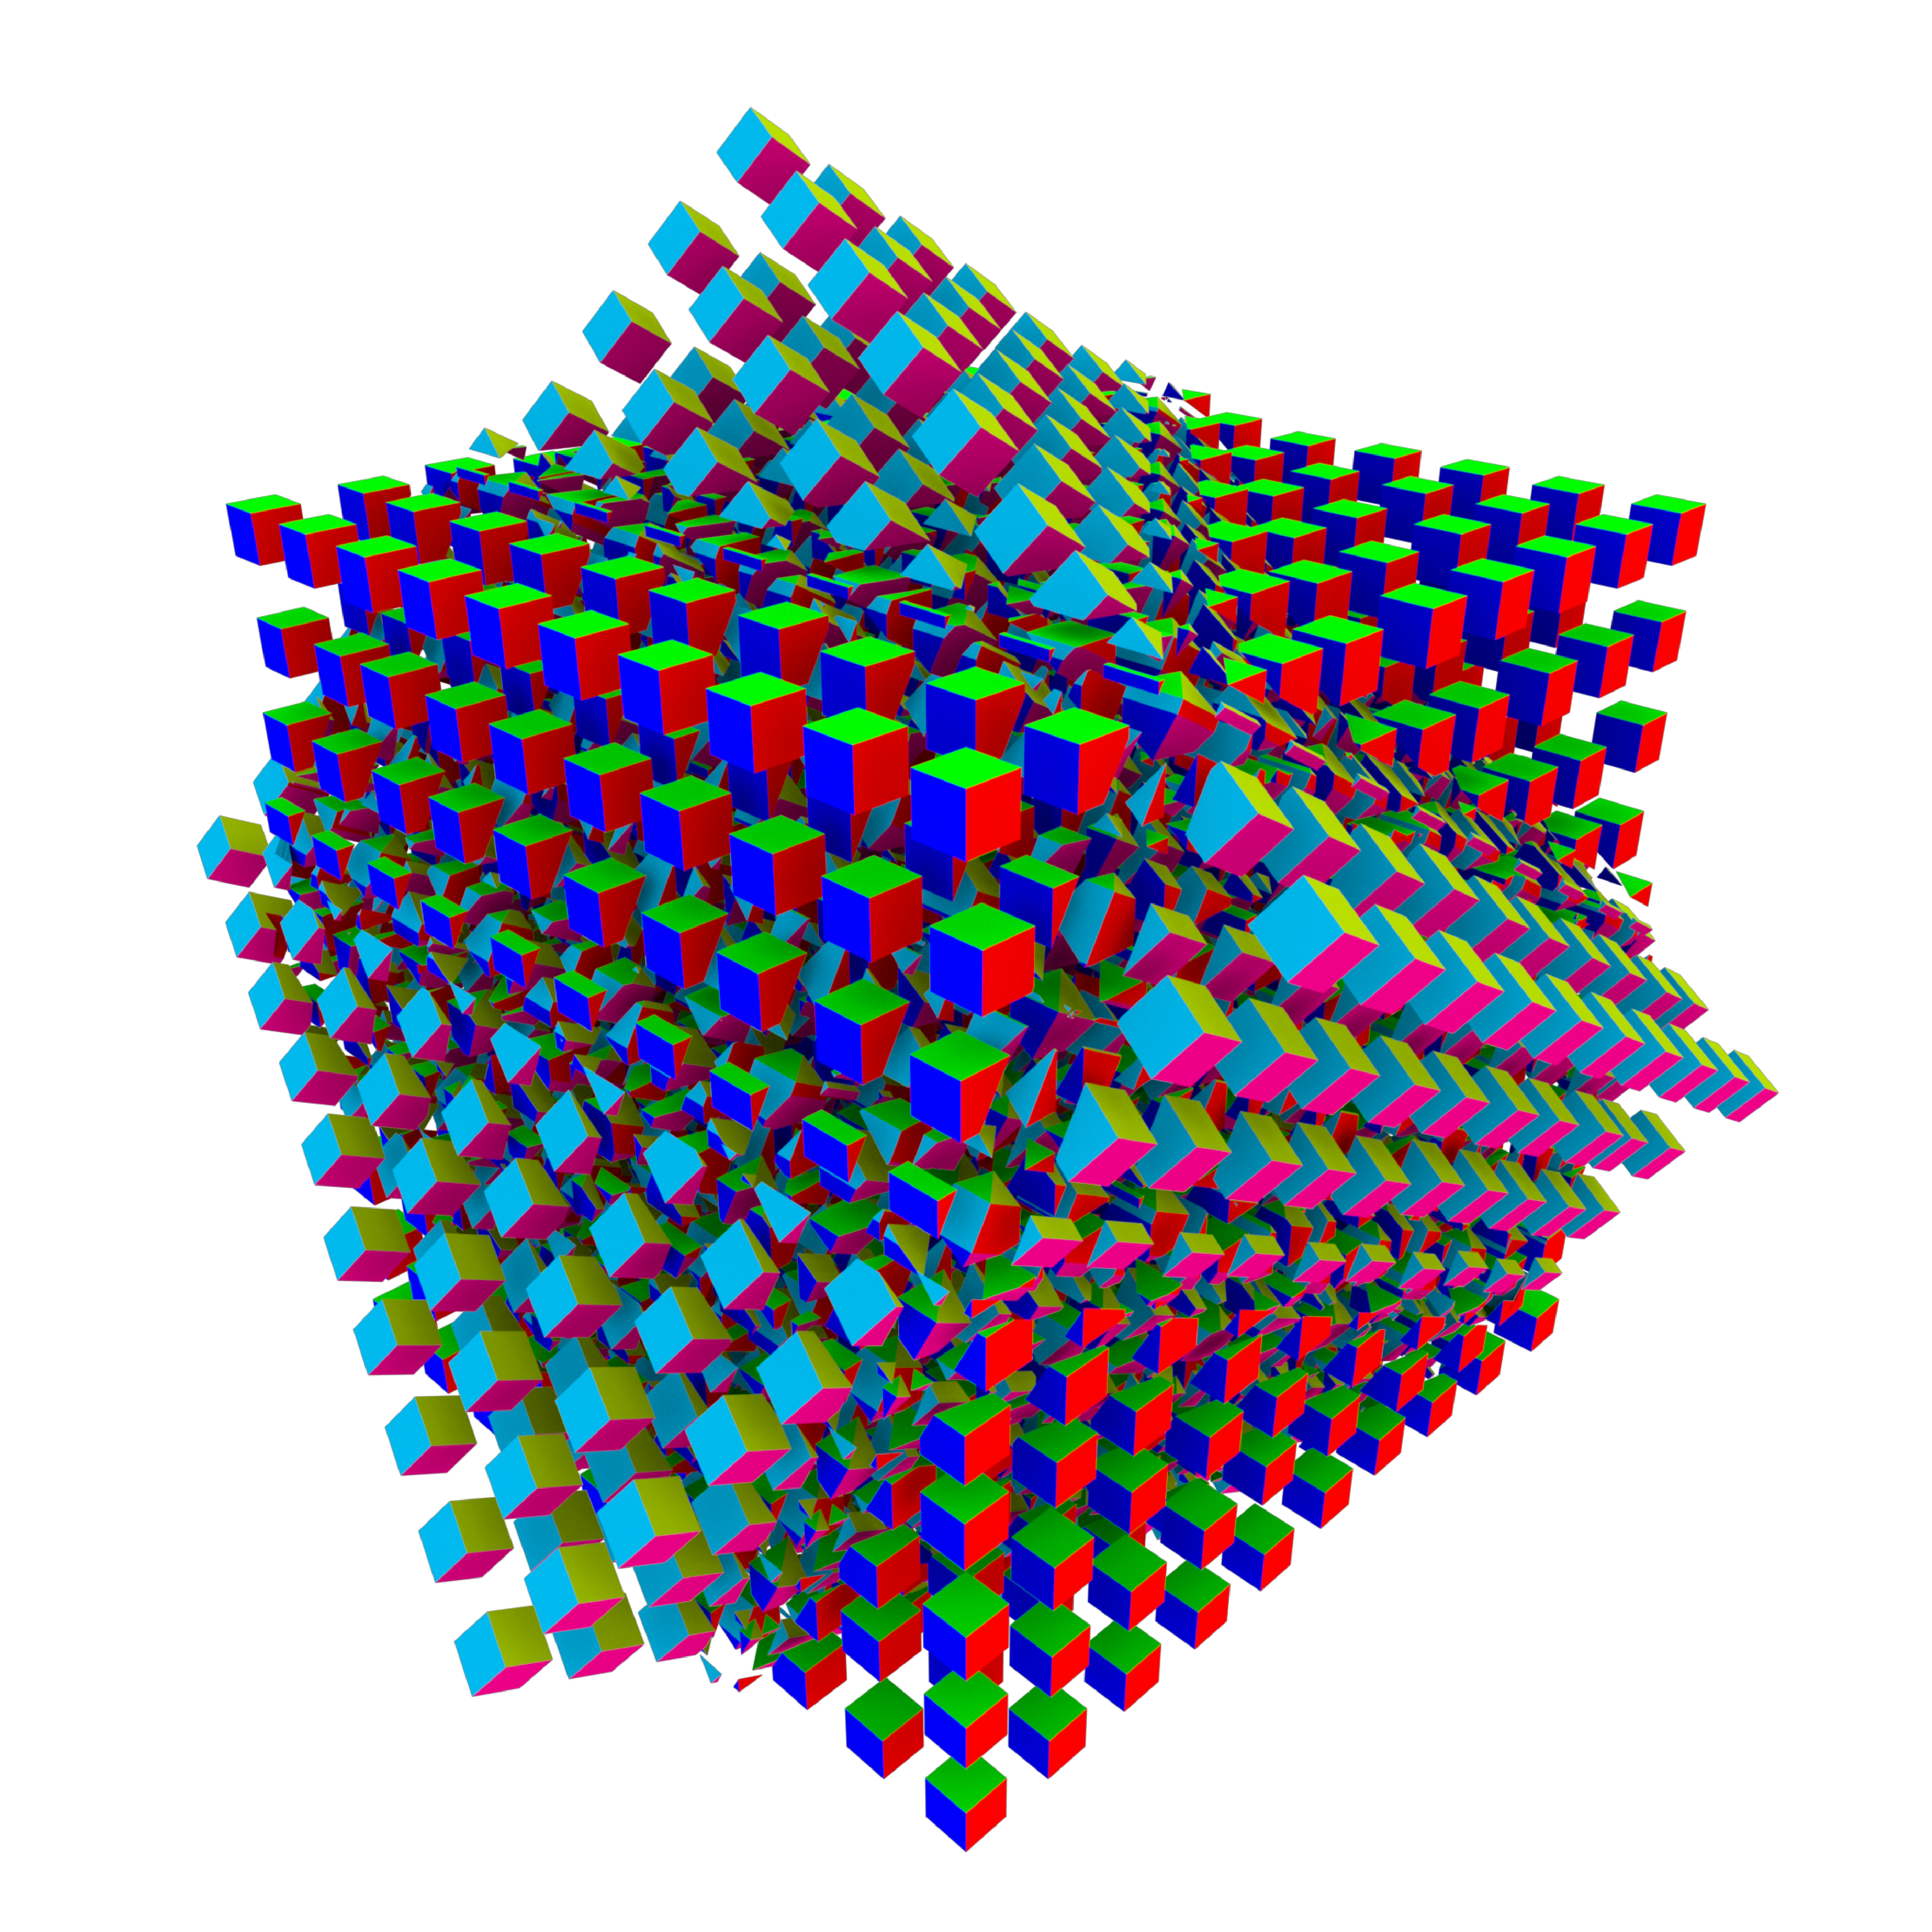
\includegraphics[width=\textwidth]{./img/cube10x10.pdf}
    \caption{Arrangement of 2000($=2\times10\times10\times10$) cubes}
\end{figure}





\section{Overview}
\label{sec:spatial_arrangement_overview}
The algorithm is based on the concept of recursive problem simplification 
(a sort of \textit{divide et impera} philosophy); if we have a $d$-complex, for every
($d-1$)-cell embedded into the $\mathbb{E}^d$ euclidean space, we bring the cell,
and every other cell that could intersect it, down into $\mathbb{E}^{d-1}$. We do this until
we reach the $d=1$ in $\mathbb{E}^1$ case; in here, we fragment all the $1$-cells.
Then, we travel back to the original $d$-dimension, and, for each
dimensional step, we build correct complexes from cells provided by the 
fragmentation of the lower dimension. 

\begin{figure}[h]
    \begin{center}
        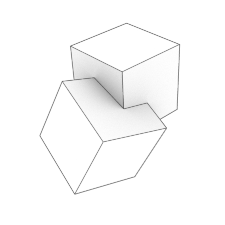
\includegraphics[width=.25\textwidth]{./img/ch1-1.pdf}%
        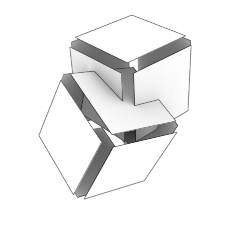
\includegraphics[width=.25\textwidth]{./img/ch1-2.pdf}%
        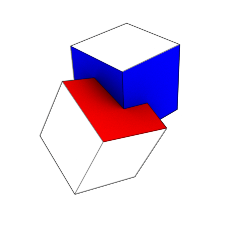
\includegraphics[width=.25\textwidth]{./img/ch1-3.pdf}%
        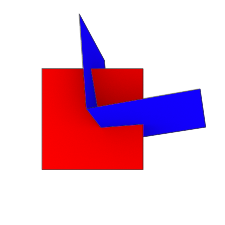
\includegraphics[width=.25\textwidth]{./img/ch1-4.pdf}%

        (a)\hspace{.22\textwidth}(b)\hspace{.22\textwidth}(c)\hspace{.22\textwidth}(d)
    \end{center}
    
    \begin{center}
        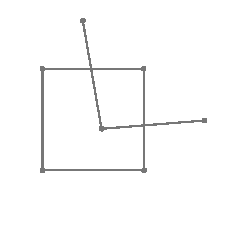
\includegraphics[width=.25\textwidth]{./img/ch1-5.pdf}%
        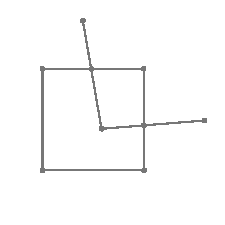
\includegraphics[width=.25\textwidth]{./img/ch1-6.pdf}%
        
\includegraphics[width=.25\textwidth]{./img/ch1-7.pdf}%
        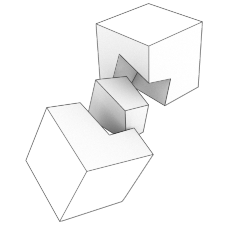
\includegraphics[width=.25\textwidth]{./img/ch1-8.pdf}%

        (e)\hspace{.22\textwidth}(f)\hspace{.22\textwidth}(g)\hspace{.22\textwidth}(h)
    \end{center}
    \caption{Algorithm overview}
    \label{img:spatial}
\end{figure}

We have in input two cellular complexes [fig. \ref{img:spatial}, a], 
given as 2-skeletons, which are the sets of 2-cells 
[fig. \ref{img:spatial}, b, exploded]. Once we merged the skeletons
[ref. \ref{sec:skel_merge}], we individuate for each $2$-cell (that we will call $\sigma$)
all the other cells that could intersect it. We do this by computing
the spatial index: it is a mapping $\mathcal{I}(\sigma)$ from a cell $\sigma$ to every other 
cell $\tau$ of which $box(\sigma) \cap box(\tau) \neq \emptyset$, where 
the $box$ function provides the axis aligned bounding box (AABB) of a cell [fig. \ref{img:spatial}, c, 
$\sigma$ in red and $\mathcal{I}(\sigma)$ in blue]. The spatial arrangement
calculation is speeded up by storing the AABBs as dimensional wise intervals
into an interval tree \cite{interval_trees}. 
Now for each cell $\sigma$ we transform $\sigma \cup \mathcal{I}(\sigma)$ 
in a way that $\sigma$ lays on the $x_3=0$ plane [fig. \ref{img:spatial}, d] and we find the intersections 
of the $\mathcal{I}(\sigma)$ cells with $x_3=0$ plane. So we have a ``soup''
of 1-cells in $\mathbb{E}^2$ [fig. \ref{img:spatial}, e], and we fragment each 1-cell 
with every other cell obtaining a valid 1-skeleton [fig. \ref{img:spatial}, f].
From this data it is possible to build the 2-cells using the ALGORITHM 1
presented and explored by Paoluzzi et al. \cite{Paoluzzi}
[fig. \ref{img:spatial}, g, exploded]. The procedure to fragment 1-cells
on a plane and return a 2-complex is called \textit{planar arrangement} and it
is presented more in detail in the next section. When the planar arrangement is
complete, fragmented $\sigma$ can be transformed back to its original position
in $\mathbb{E}^3$. With every 2-cell correctly fragmented, we can use the 
already cited ALGORITHM 1 again to build a full 3-complex%
\footnote{This is possible because ALGORITHM 1 is (almost) dimension independent
[ref. \ref{ch:minimal_cycles}].} [fig. \ref{img:spatial}, h, exploded].


\section{The ``$1$-cells in $\mathbb{E}^2$'' base case}
\label{sec:planar_arrangement_overview}

\begin{figure}[h]
    \centering
    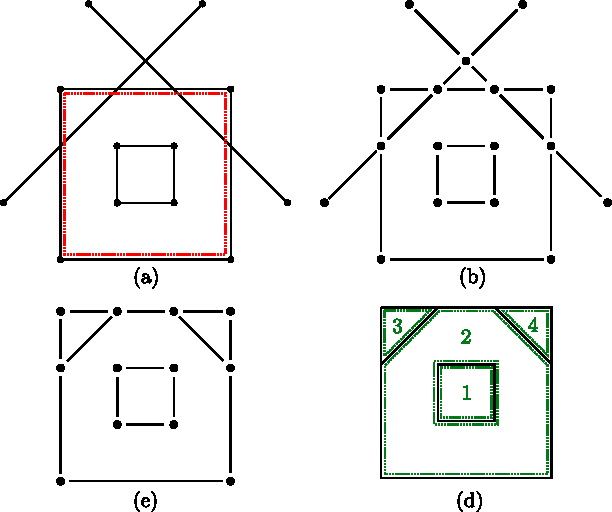
\includegraphics{./img/ch2-planararrangement.pdf}
    \caption{Planar arrangement overview}
    \label{img:planar}
\end{figure}

This is our base case. We have called \textit{planar arrangement} 
the procedure to handle this case since
it literally arranges a bunch of edges laying on a plane.
So, in input there are 1-cells in $\mathbb{E}^2$ and, optionally (but very
likely), the boundary of the original 2-cell $\sigma$ 
[fig. \ref{img:planar}, a, $\sigma$ in red].
We consider each edge and we fragment it with every other edge. This brings to
the creation of several coincident vertices: these will be eliminated
using a KD-Tree [fig. \ref{img:planar}, b, exploded]. 
At this point we have a perfectly fragmented 1-complex but many
edges are superfluous and must be eliminated; two kind of edges
are to discard: the ones outside the area of $\sigma$ and the ones
which are not part of a maximal biconnected component 
[ref. \ref{sec:biconnected_components}].
The result of this edge pruning outputs a
1-skeleton [fig. \ref{img:planar}, c, exploded].

After this, 2-cells must be computed:
for each connected component%
\footnote{It is legit to talk about a 1-skeleton as a graph: 
0-cells are nodes, 1-cells are edges and the boundary operator is
a incidence matrix.} we build a containment tree, which indicates
which component is spatially inside an other component.
Computing these relations, let us launch the ALGORITHM 1 \cite{Paoluzzi}
on each component and then combine the results to create 2-cells with non-intersecting 
shells\footnote{A 2-cell with a non-intersecting shell can be trivially defined
as a ``face with holes''; the correct definition is that it cannot 
be shrunk to the dimension of a point.} 
[fig. \ref{img:planar}, d, 2-cells numbered in green; please note that
cell 2 has cell 1 as an hole].


\section{Implementation}

Our implementation of this algorithm does not go over
$d=3$. It has been split in
multiple chapters in this book:

\begin{itemize}[noitemsep]
    \item Spatial Arrangement [ch. \ref{ch:spatial_arrangement}]: 
        It is the implementation of the ``$1$-cells in $\mathbb{E}^2$'' base case.
    \item Planar Arrangement [ch. \ref{ch:planar_arrangement}]:
        This treats the $d=3$ case. 
    \item Dimension travel [ch. \ref{ch:dimension_travel}]:
        Here are contained the utilities to travel from a
        dimension to another.
    \item Minimal cycles computation [ch. \ref{ch:minimal_cycles}]:
        This is dedicated to the implementation of the ALGORITHM 1
        described by Paoluzzi et Al. \cite{Paoluzzi}.
\end{itemize}